% Appendix D

\chapter{Pin Buffers} % Main appendix title
\label{AppendixD} % For referencing this appendix elsewhere, use \ref{AppendixA}
\lhead{Appendix D. \emph{Pin Buffers}} % This is for the header on each page - perhaps a shortened title

\begin{figure}[htbp]
\centering
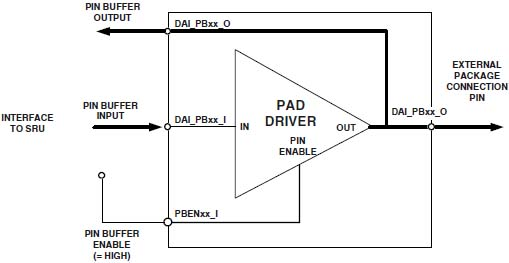
\includegraphics[height=5cm]{pinbufferOutput}
\rule{30em}{0.5pt}
\caption[Pin buffer Output]{Pin Buffer as output: pin buffer enable is logically high, the amplifier acts as a current source and drives the value at pin buffer input onto the DAI/DPI pin. Remark that pin buffer output is the same as pin buffer input and can be driven as an output.}
%\label{fig:sharc}
\end{figure}
\begin{figure}[htbp]
\centering
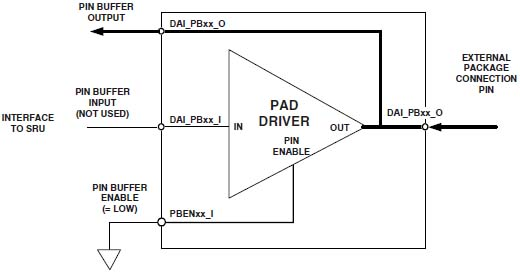
\includegraphics[height=5cm]{pinbufferInput}
\rule{30em}{0.5pt}
\caption[Pin buffer Input]{Pin Buffer as input: pin buffer enable is logically low, the amplifier disables (high output impedance) and an off-chip source can drive a value to the DAI/DPI pin via pin buffer output. In this case pin buffer input is not used.}
%\label{fig:sharc}
\end{figure}
It is recommended programming the pin buffer input logic low when the pin buffer enable is logic low. The pin buffer enable is by default connected to a SPORT pin enable signal which may change in value. By making the pin input buffer low the line is decoupled from possible irrelevant signals and code becomes easier to debug.
